\section{Theoretical Context and Motivation}
  \label{sec:theoretical-context-and-motivation}

  \subsection{Conceptual Tension Between Quantum Theory and Gravitation}
    \label{subsec:conceptual-tension-between-quantum-theory-and-gravitation}

    Quantum mechanics and general relativity differ not only in their mathematical formalisms, but also in their
    underlying conceptual foundations.
    Quantum theory is intrinsically probabilistic, relies on a fixed causal structure, and treats time as an external
    parameter\cite{Dirac1930,Born1926}.
    General relativity, by contrast, describes gravitation as the dynamics of spacetime geometry itself, with time
    emerging as a coordinate-dependent and observer-relative quantity\cite{Einstein1915,MisnerThorneWheeler1973}.

    This mismatch becomes particularly acute in regimes where both quantum effects and strong gravitational fields are
    expected to be relevant, such as near spacetime singularities or in the early universe~\cite{penrose1989emperors, prigogine1997end}.
    Attempts to quantize gravity directly often encounter conceptual obstacles, including the problem of time,
    non-renormalizability, and the absence of a preferred background structure.

    \begin{figure}[h]
      \centering
      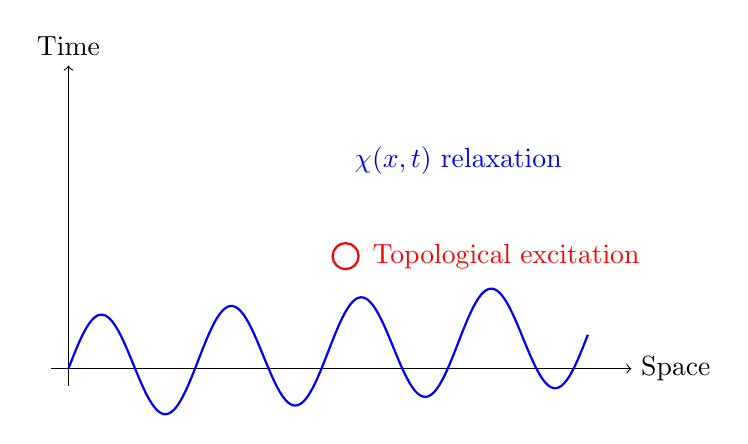
\begin{tikzpicture}[scale=1.1]

% Axes
        \draw[->] (-0.2,0) -- (6.5,0) node[right]{Space};
        \draw[->] (0,-0.2) -- (0,3.5) node[above]{Time};

% Wave
        \draw[thick, blue, domain=0:6, samples=200]
        plot (\x,{0.6*sin(2*pi*\x/1.5 r) + 0.4*\x/6});

% Particle crest
        \draw[red, thick] (3.2,1.3) circle (0.15);
        \node[red, right] at (3.4,1.3) {Topological excitation};

% Annotation
        \node[blue] at (4.5,2.4) {$\chi(x,t)$ relaxation};

      \end{tikzpicture}
      \caption{Conceptual representation of Cosmochrony. A single continuous wave field $\chi(x,t)$
        undergoes irreversible relaxation,
        characterized by a monotonic increase of its characteristic wavelength. Localized topological excitations
        correspond to particles.}
      \label{fig:chi_concept}
    \end{figure}

  \subsection{Limitations of Existing Unification Approaches}
    \label{subsec:limitations-of-existing-unification-approaches}

    Several major research programs aim to address these challenges.
    Quantum field theory in curved spacetime successfully incorporates particle creation and vacuum effects, but
    retains a classical spacetime background\cite{weinberg1972gravitation}.
    Canonical and covariant approaches to quantum gravity attempt to quantize spacetime geometry itself, often at the
    cost of mathematical complexity and interpretational ambiguity.

    String theory and related frameworks propose extended fundamental objects and higher-dimensional structures,
    offering deep mathematical unification but introducing a large landscape of possible low-energy realizations~\cite{rovelli2004quantum}.
    While these approaches are internally rich, their empirical testability remains limited, and their physical
    interpretation can be indirect.

    These considerations motivate the exploration of alternative perspectives in which spacetime geometry, matter, and
    quantum behavior are not separately postulated, but arise from a common underlying mechanism.

  \subsection{Minimalism as a Guiding Principle}\label{subsec:minimalism-as-a-guiding-principle}

    The approach developed in this work adopts minimalism as a guiding principle.
    Rather than introducing multiple fundamental fields, dimensions, or quantization rules, we consider whether a
    single continuous scalar field can encode both temporal evolution and spatial structure.

    The field $\chi(x,t)$ is not initially interpreted as a conventional matter field, nor as a metric component.
    Instead, it represents a geometric quantity whose local evolution defines both duration and separation.
    In this view, time and space are not independent primitives, but complementary aspects of the same dynamical
    process.

  \subsection{Time, Irreversibility, and Cosmological Expansion}\label{subsec:time-irreversibility-and-cosmological-expansion}

    A central motivation for the Cosmochrony framework is the close connection between time, irreversibility, and
    cosmic expansion.
    In standard cosmology, expansion is described kinematically through the scale factor, while the arrow of time is
    usually attributed to boundary conditions or entropy growth~\cite{peebles1993principles, prigogine1997end,Peebles1993,penrose1989emperors}.

    Here, the monotonic relaxation of $\chi$ provides a unified origin for both phenomena\cite{Prigogine1997}.
    Cosmological expansion corresponds to the cumulative spatial manifestation of this relaxation\cite{Peebles1993}
    , while irreversibility follows from its intrinsic directionality.
    This perspective suggests that expansion is not driven by an external energy component, but is an emergent
    geometric effect.

  \subsection{Scope and Limitations}\label{subsec:scope-and-limitations2}

    The goal of this work is exploratory rather than definitive.
    The proposed framework does not claim to replace established theories in their domains of validity, but to offer a
    coherent reinterpretation that may illuminate persistent conceptual difficulties.
    Throughout the paper, emphasis is placed on internal consistency, conceptual clarity, and contact with observable
    phenomena, while acknowledging open questions and limitations.

    In the following section, we introduce the $\chi$
    field formally and specify the minimal assumptions underlying its dynamics.
